\documentclass{article}


\title{\underline{\textbf{21 Problems}}}
\author{Aayush Bajaj}
\date{December 26, 2022}

\usepackage{tikz}
\usetikzlibrary{shapes.geometric}
\usepackage[export]{adjustbox}
\usepackage{multicol,caption}
\usepackage{graphicx}
\usepackage{fancyhdr}
\usepackage{enumitem}
\usepackage{amsmath}
\usepackage{geometry}
\geometry{
    top = 20mm,
    bottom = 35mm,
    right = 20mm,
    left = 20mm
}

\pagestyle{fancy}

\begin{document}

\maketitle

\bigbreak
\hrulefill
\bigbreak

\noindent\fbox{
    \parbox{\textwidth}{Welcome! Today is the $26^{th}$ of December, and it is my birthday :D.\\\\Today we are going to be playing a game called \textit{21 Problems}. This game consists of 21 \textbf{mathematical} problems and whoever has the highest score by midnight will be the winner!
}
}

\bigbreak
\dotfill

\section{Rules}
    \begin{enumerate}
        \item Solutions must be written on a piece of \textbf{WHITE} paper in \textbf{BLACK} pen.
            \begin{enumerate}[label*=\arabic*.]
                \item White paper can be found attached to the board in the study. Black pens are beside the board.
            \end{enumerate}
        \item To create a submission: 
            \begin{enumerate}[label*=\arabic*.]
                \item Fold the piece of paper so that your solution is \textbf{not} visible, and 
                \item Attach it to the board in the study with a magnet.
            \end{enumerate}
        \item Each submission must contain:
            \begin{enumerate}[label*=\arabic*.]
                \item Your name;
                \item The question number;
            \end{enumerate}
        \item Submissions will not be accepted after \textbf{11:59PM} on the 26th of December, 2022
        \item You may not use the \textit{internet}, but you may use any \textit{book}.
    \end{enumerate}

\section{Diagrams}

\begin{multicols}{3}
    \begin{minipage}{\linewidth}
        \centering
        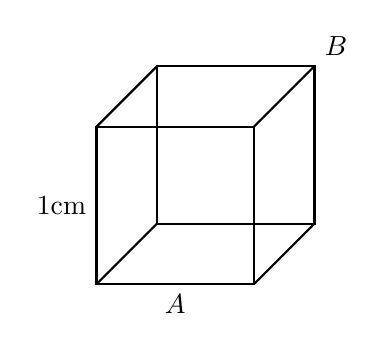
\begin{tikzpicture}
            [cube/.style={thick,black},
                grid/.style={very thin,gray},
                axis/.style={->,blue,thick}]
            %draw the top and bottom of the cube
            \draw[cube] (0,0,0) -- (0,2,0) -- (2,2,0) node[above right] {$B$} -- (2,0,0) -- cycle;
            \draw[cube] (0,0,2) -- (0,2,2)  node[left, midway]{$1\text{cm}$} -- (2,2,2) -- (2,0,2) -- node[below, midway] {$A$} cycle;
	
            %draw the edges of the cube
            \draw[cube] (0,0,0) -- (0,0,2);
            \draw[cube] (0,2,0) -- (0,2,2);
            \draw[cube] (2,0,0) -- (2,0,2);
            \draw[cube] (2,2,0) -- (2,2,2);
        \end{tikzpicture}
        \captionof*{figure}{Q4. Sugar Cube}
    \end{minipage}
    \begin{minipage}{\linewidth}
        \centering
        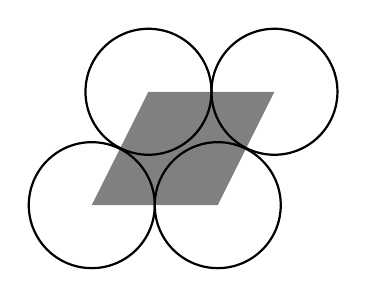
\begin{tikzpicture}[scale=0.8]
            \fill[gray] (1, 1.2) -- (3, 1.2) -- (3.9, 3) -- (1.9, 3);
            \draw[thick] (1, 1.2) circle [radius=1cm];
            \draw[thick] (3, 1.2) circle [radius=1cm];
            \draw[thick] (1.9, 3) circle [radius=1cm];
            \draw[thick] (3.9, 3) circle [radius=1cm];
        \end{tikzpicture}
        \captionof*{figure}{Q5. Hexagonal Packing}
    \end{minipage}
    \begin{minipage}{\linewidth}
        \includegraphics[width=0.7\linewidth,center]{img/implicit.png}
        \captionof*{figure}{Q18. Implicit Curve}
    \end{minipage}
\end{multicols}


\newpage{}
\fancyhead{}
\fancyfoot[L]{
    \begin{minipage}{0.25\linewidth}
        \centering
        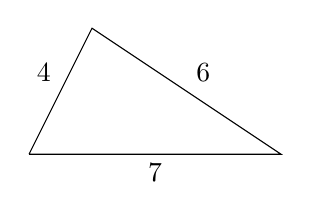
\begin{tikzpicture}[scale=0.8]
            \draw (0,0) -- (4,0) node[midway,below] {$7$}
               -- (1,2) node[midway, above right] {$6$}
               -- (0,0) node[midway, above left] {$4$};
        \end{tikzpicture}
        \captionof*{figure}{Q16. Hero's Triangle}
    \end{minipage}
}
\fancyfoot[R]{
    \begin{minipage}{0.25\linewidth}
        \centering
        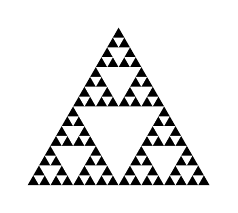
\begin{tikzpicture}[
            main tri/.style={isosceles triangle,fill,isosceles triangle apex angle=60,
                             rotate=90,inner sep=0,outer sep=0},
            filler tri/.style={isosceles triangle,fill=white,rotate=-90,isosceles triangle apex angle=60,
                             inner sep=0,outer sep=0}]
            \node[minimum height=2cm,main tri] (a) {};
            %==================
            \node[minimum height=1cm,filler tri] (b) at (a.center){};
            %==================
            \node[minimum height=0.5cm,filler tri,anchor=right corner] (c1) at (b.left side){};
            \node[minimum height=0.5cm,filler tri,anchor=left corner] (c2) at (b.right side){};
            \node[minimum height=0.5cm,filler tri,anchor=apex] (c3) at (b.west){};
            % ===================
            \foreach \x in {1,2,3}{
            \node[minimum height=0.25cm,filler tri,anchor=right corner] (d1\x) at (c\x.left side){};
            \node[minimum height=0.25cm,filler tri,anchor=left corner] (d2\x) at (c\x.right side){};
            \node[minimum height=0.25cm,filler tri,anchor=apex] (d3\x) at (c\x.west){};
            }
            % ===================
            \foreach \x in {1,2,3}{
                \foreach \y in {1,2,3}{
                \node[minimum height=0.125cm,filler tri,anchor=right corner] (e1\x\y) at (d\x\y.left side){};
                \node[minimum height=0.125cm,filler tri,anchor=left corner] (e2\x\y) at (d\x\y.right side){};
                \node[minimum height=0.125cm,filler tri,anchor=apex] (e3\x\y) at (d\x\y.west){};
                }
            }
        \end{tikzpicture}
        \captionof*{figure}{Q6. Sierpinski's Triangle}
    \end{minipage}
}
\section{Problems}

\begin{enumerate}
    \item Prove that $\frac{1}{0}$ is undefined.\hfill{}\textit{(2 marks)}
    \item Derive the identity $\sin ^2(\theta) + \cos ^2(\theta) = 1$.\hfill{}\textit{(2 marks)}
        \begin{enumerate}[label*=\arabic*.]
            \item Hence, and not otherwise, show that $1 + \cot ^2(\theta) = \csc ^2(\theta)$.\hfill{}\textit{(1 marks)}
        \end{enumerate}
    \item Find the sum of the first $1,000$ positive integers.\hfill{}\textit{(2 marks)}
    \item An ant sits on point A of $1\text{cm} \times 1\text{cm}$ sugar cube. She wants to get to point B. What is the shortest distance she can take?\hfill{}\textit{(3 marks)}
    \item What fraction of total area do the circles cover if the circles have a radius of 1.\hfill{}\textit{(3.5 marks)}
    \item What is the dimension of Sierpinski's triangle?\hfill{}\textit{(4 marks)}
    \item Prove that $\sqrt{2}$ is irrational.\hfill{}\textit{(3 marks)}
    \item Derive the quadratic formula.\hfill{}\textit{(3.5 marks)}
    \item Find the equation of the tangent and the equation of the normal to the function $f(x) = x^3 - 3x$ at the point $x = 2$.\hfill{}\textit{(4 marks)}
    \item Solve $p(x) = 2x^3 - 11x^2 +14x + 10$ if $p(3 + i) = 0$.\hfill{}\textit{(3 marks)}
    \item $\int (e^{t^2} + 16) te^{t^2} \, dt$.\hfill{}\textit{(2.5 marks)}
    \item $\int \tan (t) \sec ^2(t) \, dt$.\hfill{}\textit{(4 marks)}
    \item Sketch $\frac{1}{(x-3)(x-4)}$.\hfill{}\textit{(4 marks)}
    \item Balance the following chemical equations:
        \begin{enumerate}[label*=\arabic*.]
            \item $C_3H_8O_2 \rightarrow CO_2 + H_2O$ (combustion of propane!)\hfill{}\textit{(1 marks)}
            \item $CO_2 + H_2O \rightarrow C_6H_{12}O_6$ (photosynthesis)\hfill{}\textit{(1 marks)}
            \item $HCl + Na_3PO_4 \rightarrow H_3PO_4 + NaCl$\hfill{}\textit{(1 marks)}
        \end{enumerate}
    \item How many \textit{distinct} arrangements are there of the word \textbf{BANANA}?\hfill{}\textit{(3 marks)}
    \item Find the \underline{exact} area of the following triangle.\hfill{}\textit{(4 marks)}
    \item $\int^1_{-1} \cos(2x) + x^2 + 2^x + \frac{2}{x}\, dx$.\hfill{}\textit{(3.5 marks)}
    \item Find the equation\textit{s} of the tangent\textit{s} to $2x^3 + 2y^3 = 9xy$ at $x = 1$.\hfill{}\textit{(4.5 marks)}
    \item Glenn, the fast bowler runs in to bowl and releases the ball 2.4 metres above the ground with a speed of 144 km/h at an angle of $7^\circ$ below the horizontal. Take $g = 10 m/s^2$ and find how long before the ball hits the pitch.\hfill{}\textit{(5 marks)}
    \item Let $\vec{u} = (4,-1), \, \vec{v} = (0,5), \, \vec{w} = (-3,-3)$:
        Find:
        \begin{enumerate}[label*=\arabic*.]
            \item $\vec{u} + \vec{w}$\hfill{}\textit{(1 marks)}
            \item $\left| \vec{u} + \vec{w} \right|$\hfill{}\textit{(1 marks)}
            \item $3\vec{v} - 2\vec{u} + \vec{v}$\hfill{}\textit{(2 marks)}
        \end{enumerate}
    \item Solve the values of $x$ which satisfy the equation $23x \equiv 11 (\text{mod }30)$.\hfill{}\textit{(3 marks)}
\end{enumerate}



\end{document}
